\documentclass[landscape]{article}
\usepackage[paperwidth=254mm,paperheight=452mm,margin=0mm]{geometry}
\usepackage{tikz}
\usetikzlibrary{calc,calendar}
\usepackage{fontspec}
\usepackage{xeCJK}
\usepackage{fancyhdr}
\usepackage{pgfcalendar}
\usepackage{amssymb}
\usepackage{hyperref}

% ハイパーリンク設定
\hypersetup{
    colorlinks=true,
    linkcolor=blue,
    urlcolor=blue,
    pdfborder={0 0 0}
}

% フォント設定
\setmainfont{DejaVu Sans}
\setCJKmainfont{Noto Sans CJK JP}
\setCJKsansfont{Noto Sans CJK JP}

% ヘッダー・フッター設定
\pagestyle{fancy}
\fancyhf{}
\renewcommand{\headrulewidth}{0pt}
\renewcommand{\footrulewidth}{0pt}

% 色設定
\definecolor{lightgray}{RGB}{240,240,240}
\definecolor{medgray}{RGB}{200,200,200}
\definecolor{darkgray}{RGB}{100,100,100}
\definecolor{accent}{RGB}{100,150,200}

\setlength{\parindent}{0pt}
\setlength{\parskip}{0pt}

% 月名
\def\monthname#1{%
  \ifcase#1\or January\or February\or March\or April\or May\or June\or 
  July\or August\or September\or October\or November\or December\fi%
}

% 曜日名(短縮形)
\def\dayname#1{%
  \ifcase#1 Mon\or Tue\or Wed\or Thu\or Fri\or Sat\or Sun\fi%
}

% 曜日名(完全形)
\def\dayfulname#1{%
  \ifcase#1 Monday\or Tuesday\or Wednesday\or Thursday\or Friday\or Saturday\or Sunday\fi%
}

\begin{document}

% ========================================
% PART 1: 12 Monthly Calendars
% ========================================
\foreach \month in {1,2,...,12} {
  \hypertarget{monthly-\month}{}
  \begin{tikzpicture}[remember picture,overlay]
  \node[anchor=north west] at (current page.north west) {
  \begin{minipage}[t][452mm][t]{254mm}
  
  % ヘッダー
  \begin{tikzpicture}
  \fill[accent!30] (0,0) rectangle (254mm,32mm);
  \node[anchor=west,font=\fontsize{36}{40}\selectfont\bfseries] at (10mm,16mm) {\monthname{\month} 2025};
  \pgfcalendardatetojulian{2025-\month-01}{\startjulian}
  \pgfcalendarjuliantoweek{\startjulian}{\startyear}{\startweek}
  \node[anchor=east,font=\fontsize{16}{20}\selectfont] at (244mm,16mm) {\hyperlink{weekly-\startweek}{Weekly} | \hyperlink{daily-2025-\ifnum\month<10 0\fi\month-01}{Daily}};
  \end{tikzpicture}
  
  \vspace{5mm}
  
  % カレンダーグリッド
  \begin{tikzpicture}[x=1mm,y=1mm]
  % 曜日ヘッダー(月曜始まり)
  \foreach \x/\day in {0/Mon,1/Tue,2/Wed,3/Thu,4/Fri,5/Sat,6/Sun} {
    \pgfmathsetmacro{\xpos}{10+\x*34.57}
    \pgfmathsetmacro{\xposend}{10+(\x+1)*34.57}
    \pgfmathsetmacro{\xcenter}{\xpos+17.285}
    \fill[lightgray] (\xpos,377) rectangle (\xposend,398);
    \draw[thick] (\xpos,377) rectangle (\xposend,398);
    \node[font=\fontsize{16}{20}\selectfont\bfseries] at (\xcenter,387.5) {\day};
  }
  
  % 月の日数を取得
  \pgfcalendardatetojulian{2025-\month-01}{\julianstart}
  \pgfcalendarjuliantodate{\julianstart}{\year}{\thismonth}{\day}
  \pgfcalendarjuliantoweekday{\julianstart}{\dow}
  
  % 月曜日を0とするため調整(pgfcalendarは日曜=0)
  \pgfmathtruncatemacro{\dowmonday}{mod(\dow+6,7)}
  
  % その月の日数
  \ifnum\month=2
    \def\maxday{28}
  \else
    \ifnum\month=4
      \def\maxday{30}
    \else\ifnum\month=6
      \def\maxday{30}
    \else\ifnum\month=9
      \def\maxday{30}
    \else\ifnum\month=11
      \def\maxday{30}
    \else
      \def\maxday{31}
    \fi\fi\fi\fi
  \fi
  
  % カレンダーグリッド描画
  \foreach \row in {0,1,...,5} {
    \foreach \col in {0,1,...,6} {
      \pgfmathsetmacro{\y}{377-(\row+1)*58.67}
      \pgfmathsetmacro{\yend}{\y+58.67}
      \pgfmathsetmacro{\xpos}{10+\col*34.57}
      \pgfmathsetmacro{\xposend}{10+(\col+1)*34.57}
      \pgfmathtruncatemacro{\cellnum}{\row*7+\col}
      \pgfmathtruncatemacro{\daynum}{\cellnum-\dowmonday+1}
      
      \draw[thick] (\xpos,\y) rectangle (\xposend,\yend);
      
      % 日付表示
      \ifnum\daynum>0
        \ifnum\daynum<\maxday+1
          \node[anchor=north west,font=\fontsize{14}{16}\selectfont] at ({\xpos+2},{\yend-2}) {
            \hyperlink{daily-2025-\ifnum\month<10 0\fi\month-\ifnum\daynum<10 0\fi\daynum}{\daynum}
          };
        \fi
      \fi
    }
  }
  \end{tikzpicture}
  
  \end{minipage}
  };
  \end{tikzpicture}
  
  \newpage
}

% ========================================
% PART 2: 54 Weekly Schedules (Week 1-54 of 2025)
% ========================================
\foreach \week in {1,2,...,54} {
  % 週の開始日(月曜日)を計算
  \pgfcalendarweekdaytojulian{\week}{1}{2025}{\julianmonday}
  \pgfcalendarjuliantodate{\julianmonday}{\year}{\startmonth}{\startday}
  
  % 週の終了日(日曜日)を計算
  \pgfmathtruncatemacro{\juliansunday}{\julianmonday+6}
  \pgfcalendarjuliantodate{\juliansunday}{\endyear}{\endmonth}{\endday}
  
  \hypertarget{weekly-\week}{}
  \begin{tikzpicture}[remember picture,overlay]
  \node[anchor=north west] at (current page.north west) {
  \begin{minipage}[t][452mm][t]{254mm}
  
  % ヘッダー
  \begin{tikzpicture}
  \fill[accent!30] (0,0) rectangle (254mm,32mm);
  \node[anchor=west,font=\fontsize{36}{40}\selectfont\bfseries] at (10mm,16mm) {Week \week: \monthname{\startmonth} \startday{} - \monthname{\endmonth} \endday};
  \node[anchor=east,font=\fontsize{16}{20}\selectfont] at (244mm,16mm) {
    \hyperlink{monthly-\startmonth}{Monthly} | 
    \hyperlink{daily-\year-\ifnum\startmonth<10 0\fi\startmonth-\ifnum\startday<10 0\fi\startday}{Daily}
  };
  \end{tikzpicture}
  
  \vspace{5mm}
  
  % 時間軸付き週間表
  \begin{tikzpicture}[x=1mm,y=1mm]
  % 曜日ヘッダー(月曜始まり)
  \foreach \d in {0,1,...,6} {
    \pgfmathtruncatemacro{\currentjulian}{\julianmonday+\d}
    \pgfcalendarjuliantodate{\currentjulian}{\cyear}{\cmonth}{\cday}
    \pgfcalendarjuliantoweekday{\currentjulian}{\cdow}
    
    \pgfmathsetmacro{\xpos}{10+\d*34.57}
    \pgfmathsetmacro{\xposend}{10+(\d+1)*34.57}
    \pgfmathsetmacro{\xcenter}{\xpos+17.285}
    
    \fill[lightgray] (\xpos,380) rectangle (\xposend,396);
    \draw[thick] (\xpos,380) rectangle (\xposend,396);
    
    \node[font=\fontsize{14}{18}\selectfont\bfseries] at (\xcenter,390) {\dayname{\d}};
    \node[font=\fontsize{12}{14}\selectfont] at (\xcenter,384) {
      \hyperlink{daily-\cyear-\ifnum\cmonth<10 0\fi\cmonth-\ifnum\cday<10 0\fi\cday}{\cmonth/\cday}
    };
  }
  
  % 時間軸と罫線
  \foreach \h in {6,7,...,23} {
    \pgfmathsetmacro{\y}{380-(\h-6)*21.1}
    \draw[medgray] (10,\y) -- (252,\y);
    \node[anchor=east,font=\fontsize{12}{14}\selectfont] at (9,\y) {\h:00};
  }
  
  % 縦線(曜日の区切り)
  \foreach \x in {0,1,...,7} {
    \pgfmathsetmacro{\xpos}{10+\x*34.57}
    \draw[thick] (\xpos,0) -- (\xpos,396);
  }
  
  % 外枠
  \draw[very thick] (10,0) rectangle (252,396);
  \end{tikzpicture}
  
  \end{minipage}
  };
  \end{tikzpicture}
  
  \newpage
}

% ========================================
% PART 3: 365 Daily Planners
% ========================================
\foreach \dayofyear in {1,2,...,365} {
  % ユリウス日から日付を計算
  \pgfcalendardatetojulian{2025-01-01}{\julianstart}
  \pgfmathtruncatemacro{\currentjulian}{\julianstart+\dayofyear-1}
  \pgfcalendarjuliantodate{\currentjulian}{\year}{\month}{\day}
  \pgfcalendarjuliantoweekday{\currentjulian}{\dow}
  \pgfcalendarjuliantoweek{\currentjulian}{\wYear}{\weeknum}
  
  % 月曜日を0とする
  \pgfmathtruncatemacro{\dowmonday}{mod(\dow+6,7)}
  
  \hypertarget{daily-\year-\ifnum\month<10 0\fi\month-\ifnum\day<10 0\fi\day}{}
  \begin{tikzpicture}[remember picture,overlay]
  \node[anchor=north west] at (current page.north west) {
  \begin{minipage}[t][452mm][t]{254mm}
  
  % ヘッダー
  \begin{tikzpicture}
  \fill[accent!30] (0,0) rectangle (254mm,32mm);
  \node[anchor=west,font=\fontsize{36}{40}\selectfont\bfseries] at (10mm,16mm) {
    \dayfulname{\dowmonday}, \monthname{\month} \day
  };
  \node[anchor=east,font=\fontsize{16}{20}\selectfont] at (244mm,16mm) {
    \hyperlink{monthly-\month}{Monthly} | \hyperlink{weekly-\weeknum}{Weekly}
  };
  \end{tikzpicture}
  
  \vspace{5mm}
  
  % 左側:時間割
  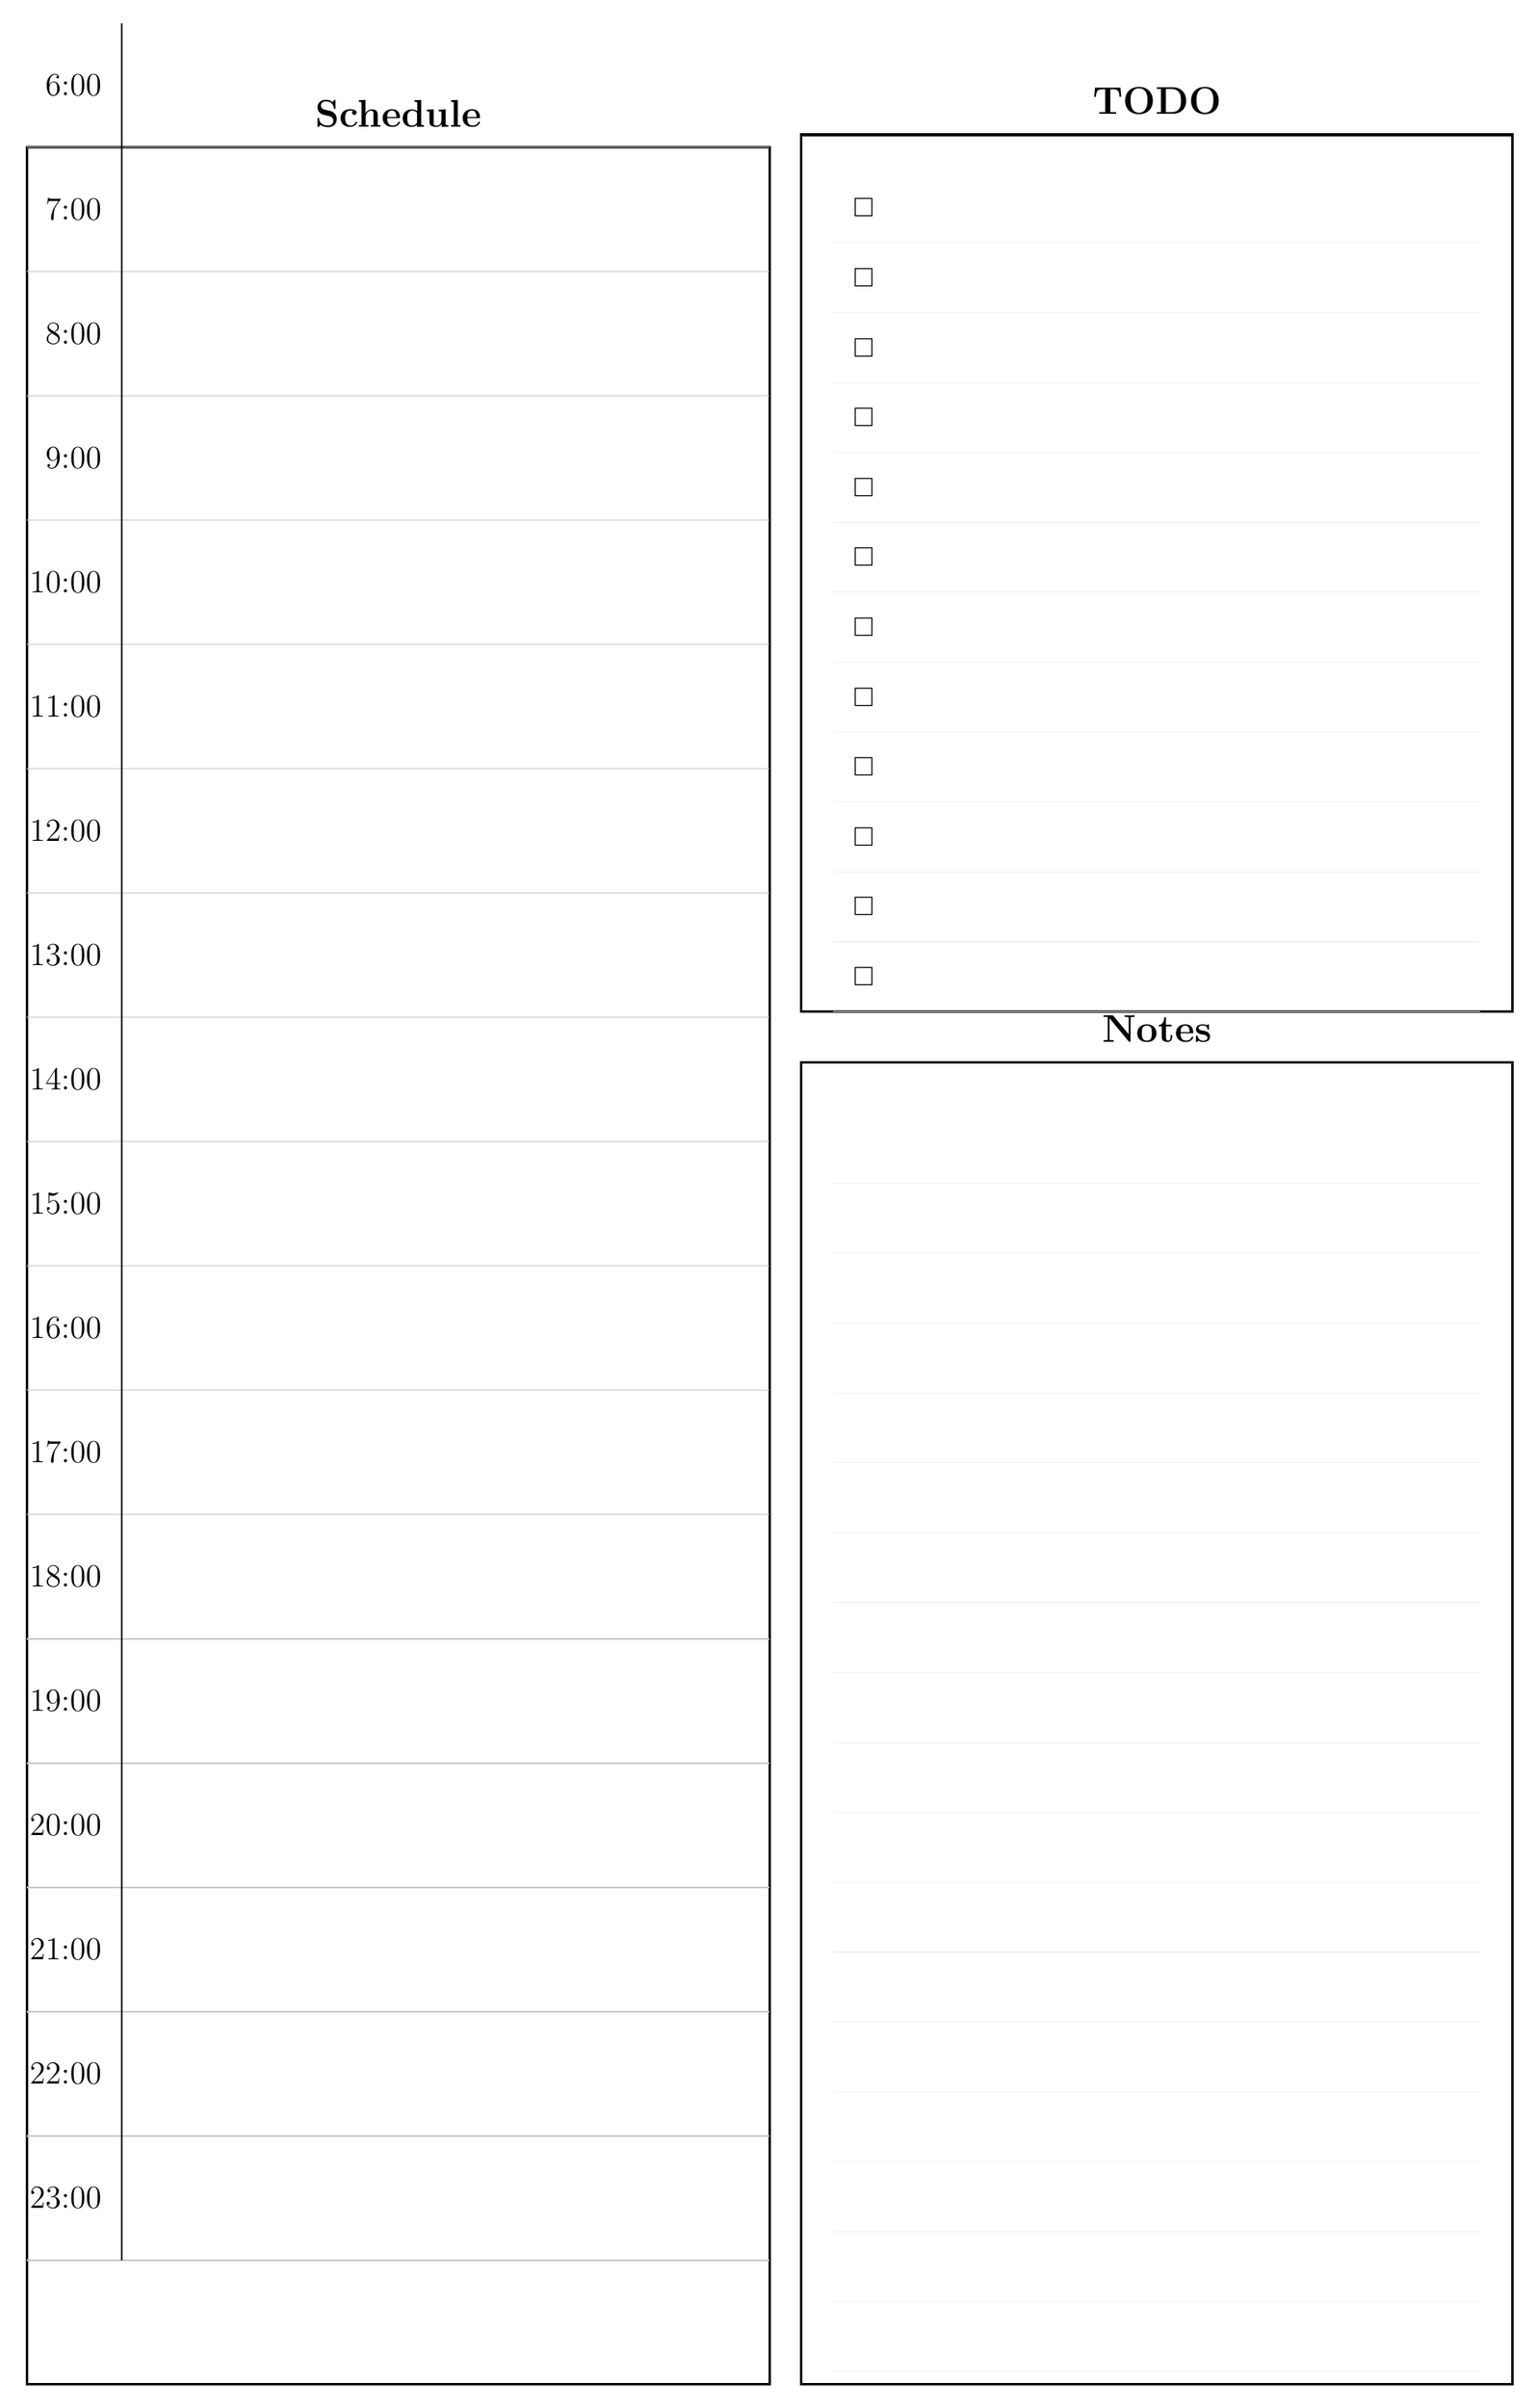
\begin{tikzpicture}[x=1mm,y=1mm]
  \draw[very thick] (10,20) rectangle (127,372);
  \node[anchor=south,font=\fontsize{16}{20}\selectfont\bfseries] at (68.5,374) {Schedule};
  
  \foreach \h in {6,7,...,23} {
    \pgfmathsetmacro{\y}{372-(\h-6)*19.56}
    \pgfmathsetmacro{\yend}{\y+19.56}
    \pgfmathsetmacro{\ycenter}{\y+9.78}
    \draw[medgray] (10,\y) -- (127,\y);
    \node[anchor=east,font=\fontsize{14}{16}\selectfont] at (23,\ycenter) {\h:00};
    \draw[thick] (25,\y) -- (25,\yend);
  }
  
  % 右側:TODO & Notes
  \draw[very thick] (132,236) rectangle (244,374);
  \node[anchor=south,font=\fontsize{16}{20}\selectfont\bfseries] at (188,376) {TODO};
  
  \foreach \i in {1,2,...,12} {
    \pgfmathsetmacro{\y}{368-\i*11}
    \pgfmathsetmacro{\ycenter}{\y+5.5}
    \draw[lightgray] (137,\y) -- (239,\y);
    \node[anchor=west,font=\fontsize{12}{14}\selectfont] at (139,\ycenter) {$\square$};
  }
  
  % Notesエリア
  \draw[very thick] (132,20) rectangle (244,228);
  \node[anchor=south,font=\fontsize{16}{20}\selectfont\bfseries] at (188,230) {Notes};
  
  \foreach \i in {1,2,...,18} {
    \pgfmathsetmacro{\y}{220-\i*11}
    \draw[lightgray] (137,\y) -- (239,\y);
  }
  \end{tikzpicture}
  
  \end{minipage}
  };
  \end{tikzpicture}
  
  \newpage
}

\end{document}